\subsection{\textbf{Das} Beispiel}
\begin{frame}
	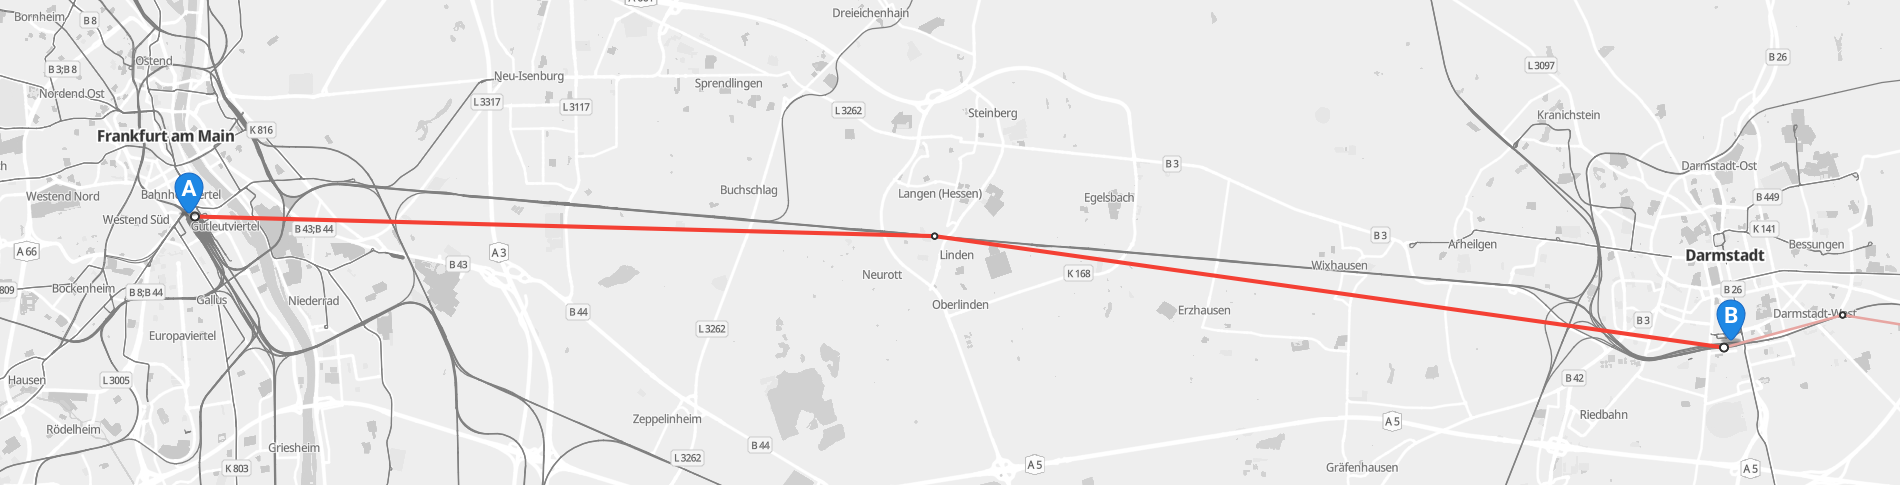
\includegraphics[width=\linewidth]{images/bahnstrecke-frankfurt-darmstadt.png}

	\hspace{5em}

	\begin{itemize}
		\item Quelle: \url{europe.motis-project.de} [Super bei Verspätungen ;)]
	\end{itemize}
\end{frame}

\subsection{Das Problem}
\begin{frame}
	\vspace{6em}
	\begin{center}
		\begin{Large}
			Wie muss ich meinen Graph modellieren, damit ich das Earliest Arrival Problem mit einem Shortest Path Algorithmus lösen kann?
		\end{Large}
	\end{center}
\end{frame}

\begin{frame}{1. Griff in die Terminologie-Kiste}
	\framesubtitle{Züge und Stationen}

	\begin{block}{}
		Züge und Zugklassen
	\end{block}
	
	\begin{center}
		\begin{tikzpicture}
			\node (img1) {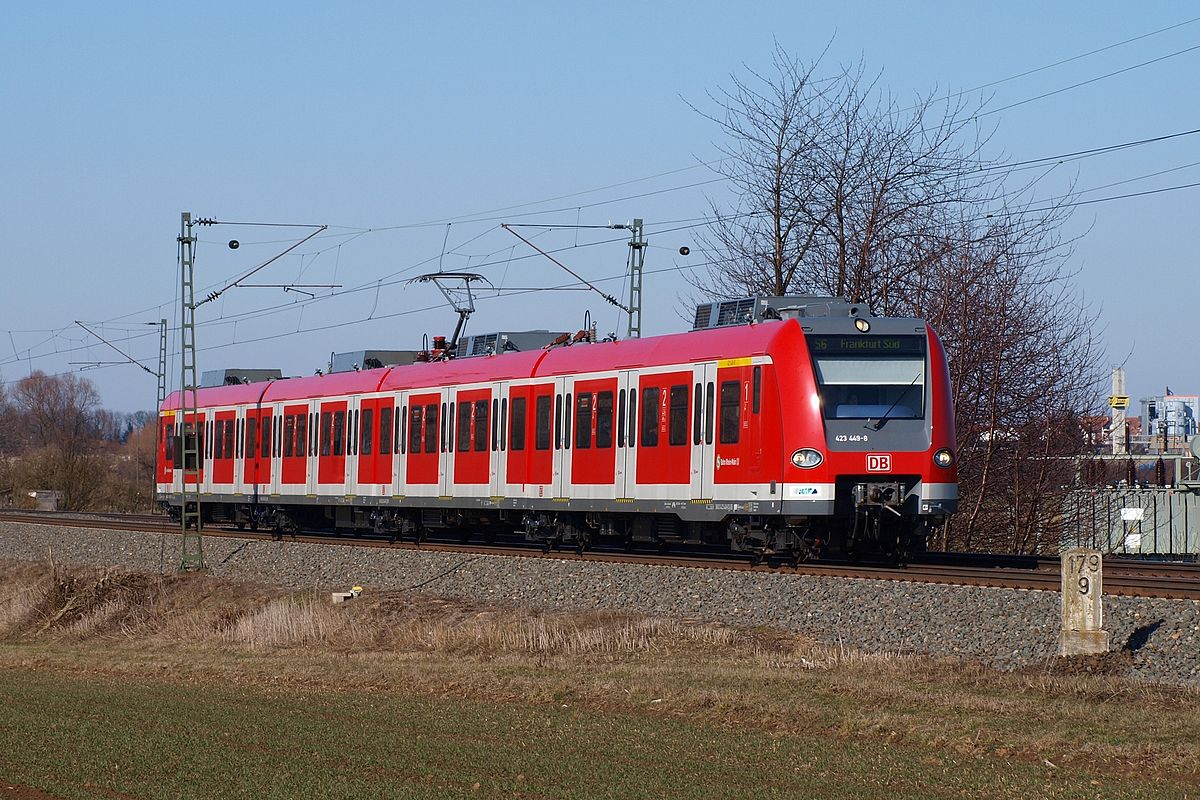
\includegraphics[height=4.5cm]{images/sbahn.jpg}};
			\pause
			\node (img2) at (img1.center) {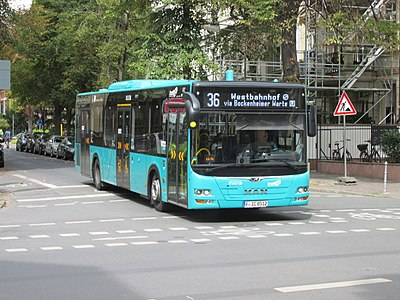
\includegraphics[height=4.5cm]{images/bus.jpg}};
			\pause
			\node (img3) at (img2.center) {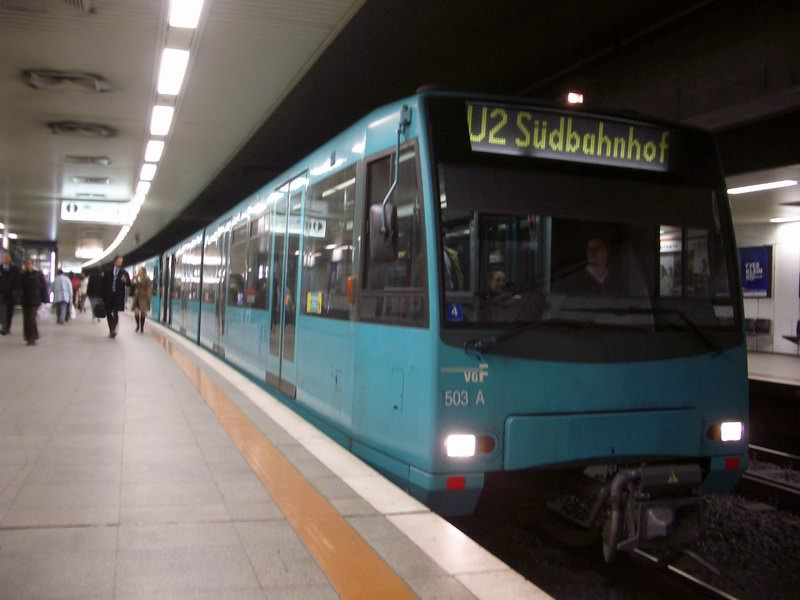
\includegraphics[height=4.5cm]{images/ubahn.jpg}};
			\pause
			\node (img4) at (img3.center) {\includegraphics[height=4.5cm]{images/fähre.jpg}};
		\end{tikzpicture}
	\end{center}
\end{frame}

\begin{frame}{1. Griff in die Terminologie-Kiste}
	\framesubtitle{Züge und Stationen}

	\begin{block}{}
		Stationen
	\end{block}
	
	\begin{center}
		\begin{tikzpicture}
			\node (img1) {\includegraphics[height=4.5cm]{images/köppern.jpg}};
			\pause
			\node (img2) at (img1.center) {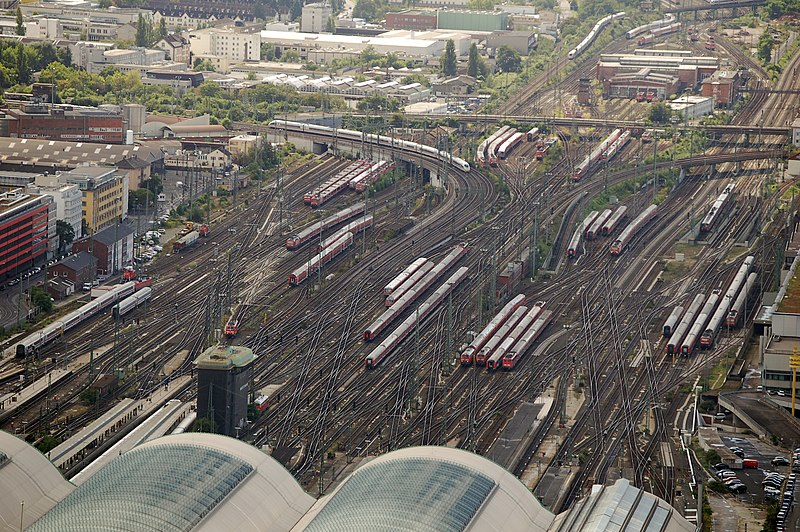
\includegraphics[height=4.5cm]{images/ffm.jpg}};
		\end{tikzpicture}
	\end{center}
\end{frame}


\subsection{Naive Ansätze}
\begin{frame}{Wie modelliere ich einen Fahrplan als Graphen?}
	\begin{itemize}
		\item Simple Idee: Nodes sind Stationen, Edges sind Verbindungen 
	\end{itemize}
	
	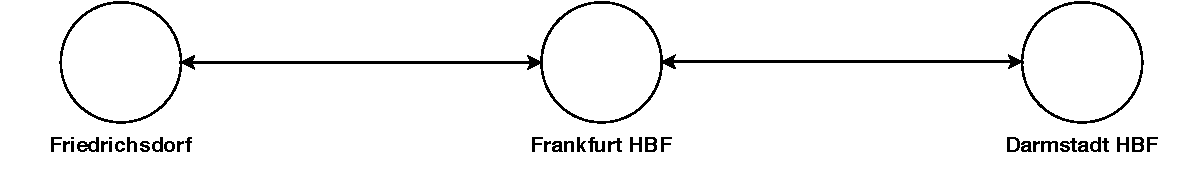
\includegraphics[width=\linewidth]{images/simple-approach.pdf} \pause

	\begin{block}{}
		Was ist das Problem hier?
	\end{block}
\end{frame}

\begin{frame}
	\begin{itemize}
		\item Wir müssen irgendwie Zeitverhältnisse innerhalb des Graphen darstellen!
	\end{itemize}
	
	\begin{center}
		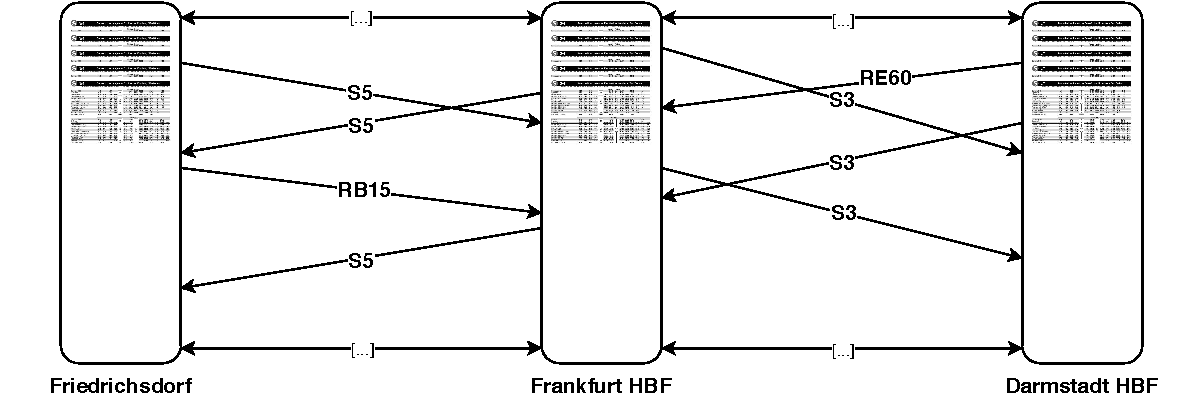
\includegraphics[width=\linewidth]{images/simple-approach-timed.pdf}
	\end{center}
\end{frame}

\begin{frame}
	\begin{itemize}
		\item Wir müssen irgendwie Zeitverhältnisse innerhalb des Graphen darstellen!
	\end{itemize}
	
	\begin{center}
		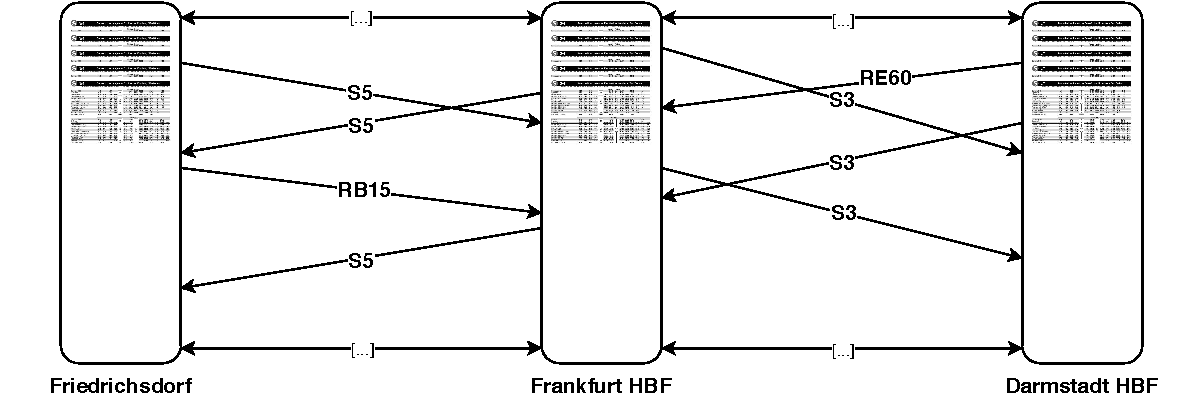
\includegraphics[width=\linewidth]{images/simple-approach-timed-2.pdf} \pause
	\end{center}

	\begin{block}{}
		Was ist das Problem hier?
	\end{block}
\end{frame}

\begin{frame}{Probleme}
	\framesubtitle{Die es zu lösen gilt...}
	\begin{itemize}
		\item Zeitverhältnisse im Graphen \pause
		\item \textbf{Takt}fahrpläne \pause
		\item Umstiege bzw. Umsteigezeiten \pause		
		\item Fußwege zwischen / innerhalb von Stationen \pause
		\item Intermodalität
	\end{itemize}
	
	\vspace{3em}
	\begin{block}{Zwei gängige Modelle}
		Time-Expanded vs. Time-Dependent
	\end{block}
\end{frame}


\begin{frame}{Größenordnungen}
	\begin{itemize}
		\item Ein paar Zahlen im Jahr 2008 (\textbf{nur} Züge):
	\end{itemize}

	\begin{center}
		\begin{tabular}{ c|c } 
			Anzahl an & \\
 			\hline
 			Zügen & 68073 \\ 
 			Fußwegen & 425
		\end{tabular}
	\end{center}
\end{frame}



















